\documentclass[12pt]{article}


\usepackage[dvips,letterpaper,margin=0.75in,bottom=0.75in]{geometry}
\usepackage{cite}
\usepackage{slashed}
\usepackage{graphicx}
\usepackage{amsmath}

\usepackage[american,fulldiode]{circuitikz}

\begin{document}
\ctikzset{bipoles/thickness=1}
\ctikzset{bipoles/length=.6cm}

\title{Lab 1:  The Transistor}

\maketitle

\section{Pre-lab Calculations}
\noindent
1) Calculate the expected gain for the circuit in Fig.~\ref{fig:follower}.   Assume the capacitance $C$ is infinitely large, so that you can neglect the voltage divider at the input.\\

\noindent
2) Calculate the expected gain for the circuit in Fig.~\ref{fig:amp}.  Assume the capacitance $C$ is infinitely large, so that you can neglect the voltage divider at the input.

\section{Introduction}

In this lab, you will build three common circuits which make use of transistor:  a transistor switch, an emitter follower, and a common-emitter amplifier.  You will measure their performance and compare with the design parameters.

\section{Transistor Switch}

\begin{figure}[htbp]
\begin{center}
\begin{tabular}{c@{\hskip 2cm}c}
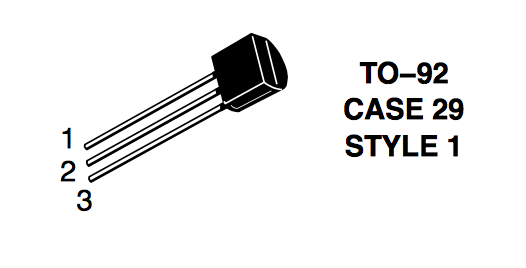
\includegraphics[height=0.10\textheight]{figs/case3904.png} &
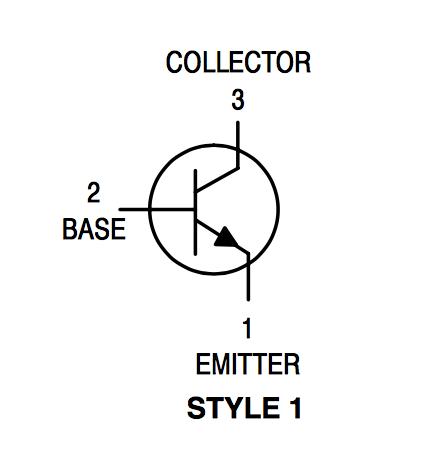
\includegraphics[height=0.18\textheight]{figs/chan3904.png} \\
\end{tabular}
\end{center}
\caption{The TO-92 Style 1 package used for some discrete transistors, including the 2N3904 transistor used throughout this lab.  Note that not all transistors use the same pinout, even if they are in the TO-92 package.}
\label{fig:layout}
\end{figure}

\begin{figure}[htbp]
\begin{center}
\begin{tabular}{c@{\hskip 2cm}c}
\begin{circuitikz}[line width=1pt]
\draw
(0,0) to[square voltage source,bipoles/length=1.5cm,l=$v(t)$] (0,5) -- ++(2,0)
to[resistor,l_=$R_1$] ++(0,-1.5)  to[diode,l_=$D$] ++(0,-1) to[short,-*] (2,0)-- (0,0)
(2,0) node[ground,yscale=2.0]{}
;
% hack for LED... automatic arrows look terrible.
\draw[->] (2.2,3.0) -- (2.4,2.8);
\draw[->] (2.3,3.2) -- (2.5,3.0);
\end{circuitikz} &

\begin{circuitikz}[line width=1pt]
\draw
(0,0) node[npn](npn1){} 
(npn1.E) to ++(0,-1.25) coordinate (A) node[ground,yscale=2.0]{}
(npn1.B) to [R,l_=$R_2$] ++(-1.5,0)  to[square voltage source,bipoles/length=1.5cm,l_=$v(t)$] ++(0,-2) 
to[short,-*] (A) 
(npn1.C)+(0,2) coordinate (B)
node[right]{$V_{\rm CC}$}
(B) to[resistor,l_=$R_1$,o-] ++(0,-1.5) to[diode,l_=$D$] (npn1.C)
;
% hack for LED... automatic arrows look terrible.
\draw[->] (0.2,1.0) -- (0.4,0.8);
\draw[->] (0.3,1.2) -- (0.5,1.0);
\end{circuitikz} \\
(a) & (b) \\
\end{tabular}
\caption{Circuits for driving an LED (a) directly from the signal voltage and (b) using a diode switch.}
\label{fig:ledcircuits}
\end{center}
\end{figure}

In this section you will build a diode switch to control a light emitting diode (LED).  You will use a 2N3904 NPN transistor in the TO-92 Style 1 package as shown in Fig.~\ref{fig:layout}.

First setup the function generator to produce a square wave at a frequency of $2~\rm Hz$ with maximum voltage of $10~\rm V$ and a minimum of $0~\rm V$.  Build the circuit in Fig.~\ref{fig:ledcircuits}a using a green diode for $D$ and $R_1=820~\Omega$.  You should observe the LED blinking brightly.

If signals (in this case provided by the function generator) were always large enough to drive loads (in this case the LED and resistor) there would never be a need for amplification.  But it isn't always so easy!  
Simulate a weak signal by turning down the maximum voltage provided by the function generator to $2~\rm V$.  The LED blinking will be no longer visible.

Now build the circuit in Fig.~\ref{fig:ledcircuits}b using a  2N3904 NPN transistor, $R_1=R_2=820~\Omega$ and the same green diode.  The function generator will still provide the weak square wave $V(t)$, but provide $V_{\rm cc}=10~\rm V$ from your bench-top DC power supply.  You should now observe the LED blinking brightly again, powered by the bench-top supply, but controlled by the weak signal provided by the function generator.

\section{Emitter Follower}

\begin{figure}[htbp]
\begin{center}
\begin{circuitikz}[line width=1pt]
\draw
%(2,4) node[right]{$P_2$} to[diode,l=$D$,o-o] (2,2) node[right] {$P_1$} to[resistor,l=$R$,-o](2,0) node[right]{$G$} -- (0,0)
%(2,0) -- ++(0,0) node[ground,yscale=2.0]{}
(0,0) node[npn](npn1){} 
(npn1.B) -- ++(-0.5,0) coordinate(A) to [R,l_=$R_2$,*-] ++(0,-2) coordinate(B) 
(npn1.E) to[short,*-o] ++(1.0,0) node[right]{$v_{\rm out}$}
(npn1.E) to[R,l=$R_{\rm E}$,*-*] ++(0,-1.5) node[ground,yscale=2.0]{} -| (B)
(npn1.C) to[short,-*] ++(0,1.25) coordinate(C) to[short] ++(0,.5) node[right]{$V_{\rm CC}$}
(A) to[R,l=$R_1$] ++ (0,2) -| (C)
(npn1.C) to[short,-o] ++(0,1.75) node[right]{$V_{\rm CC}$}
(A) to[C,l=$C$,-o] ++ (-2.0,0) node[left]{$v_{\rm in}$}
;
\end{circuitikz} 
\caption{An emitter follower circuit.}
\label{fig:follower}
\end{center}
\end{figure}

\noindent
In this section, you will build the emitter follower circuit of Fig.~\ref{fig:follower}.   Use a 2N3904 NPN transistor, $R_1 = 5.6~\rm{k\Omega}$, $R_2 = 8.2~\rm k\Omega$, $R_{\rm E} = 4.7~\rm k\Omega$, 
and $C=1~\rm \mu F$. Provide $V_{\rm CC}=10~\rm V$ from your bench-top DC power supply.
The input signal $v_{\rm in}$ is provided by your function generator, initially set to provide a $10~\rm kHz$ sine wave with $V_{\rm pp} = 5~\rm V$.

Setup your oscilloscope to measure the voltage $v_{\rm in}$ and $v_{\rm out}$ simultaneously.  Use DC coupling for $v_{\rm in}$ but use AC coupling for $v_{\rm out}$.  Estimate the gain.   Using your DMM, also measure the quiescent point (DC offset) for the output $v_{\rm out}$.

Now, with both channels on the same voltage scale, chosen to be as large as possible while still displaying the entire waveform, use the scopes $XY$ mode and observe the response.  Step through different functional shapes (square, sine, arbitrary).  What is the gain?  How linear is your follower?

\section{Common Emitter Amplifier}
\begin{figure}[htbp]
\begin{center}
\begin{circuitikz}[line width=1pt]
\draw
%(2,4) node[right]{$P_2$} to[diode,l=$D$,o-o] (2,2) node[right] {$P_1$} to[resistor,l=$R$,-o](2,0) node[right]{$G$} -- (0,0)
%(2,0) -- ++(0,0) node[ground,yscale=2.0]{}
(0,0) node[npn](npn1){} 
(npn1.B) -- ++(-0.5,0) coordinate(A) to [R,l_=$R_2$,*-] ++(0,-2) coordinate(B) 
(npn1.C) to[short,*-o] ++(1.0,0) node[right]{$v_{\rm out}$}
(npn1.E) to[R,l=$R_{\rm E}$,-*] ++(0,-1.5) node[ground,yscale=2.0]{} -| (B)
(npn1.C) to[R,l_=$R_{\rm C}$,-*] ++(0,1.5) coordinate(C) to[short,-o] ++(0,.5) node[right]{$V_{\rm CC}$}
(A) to[R,l=$R_1$] ++ (0,2) |- (C)
(A) to[C,l=$C$,-o] ++ (-2.0,0) node[left]{$v_{\rm in}$}
;
\end{circuitikz} 
\caption{A common emitter amplifier.}
\label{fig:amp}
\end{center}
\end{figure}

\noindent
In this section, you will build the common emitter amplifier circuit of Fig.~\ref{fig:amp}.  Use a 2N3904 NPN transistor, $R_1 = 18~\rm{k\Omega}$, $R_2 = 3.3~\rm k\Omega$, $R_{\rm E} = 680~\rm \Omega$, $R_{\rm C} = 3.9~\rm k\Omega$ and $C=1~\rm \mu F$. Provide $V_{\rm CC}=10~\rm V$ from your bench-top DC power supply.  The input signal $v_{\rm in}$ is provided by your function generator, initially set to provide a $10~\rm kHz$ sine wave with peak-to-peak voltage $V_{\rm pp} = 1~\rm V$.

Setup your oscilloscope to measure the voltage $v_{\rm in}$ and $v_{\rm out}$ simultaneously.  Use DC coupling for $v_{\rm in}$ but use AC coupling for $v_{\rm out}$.  

Measure the gain $G = v_{\rm out}/v_{\rm in}$.  Using your DMM, also measure the quiescent point (DC offset) for the output $v_{\rm out}$.  Now setup the scope so that the input $v_{\rm in}$ has a voltage scale five times smaller than the output $v_{\rm in}$.  Use the $XY$ mode and observe the response.  What is the gain?  How linear is the amplifier?


\section{Transistor Current Source}

\begin{figure}[htbp]
\begin{center}
\begin{tabular}{c@{\hskip 0.25in}c}
\begin{circuitikz}[line width=1pt]
\draw
(0,0) node[pnp](pnp1){} 
++(-2,0) node[pnp,xscale=-1.0](pnp2){}
(pnp2.E) to[short,-*] (pnp1.E) to [short,-o] ++(0,0.5) node[right]{$V_+$}
(pnp1.B) to[short] ($(pnp1.B)!0.5!(pnp2.B)$) coordinate(A) to[short,*-] (pnp2.B)
(A) |- (pnp1.C) to[R,l=$R_{\rm P}$,*-] ++(0,-1.5) node[ground,yscale=2.0]{} 
(pnp2.C) node[left]{$P_{\rm src}$} to[R,l=$R_{\rm L}$,o-] ++(0,-1.5) node[ground,yscale=2.0]{} 
;
\end{circuitikz} &
\begin{circuitikz}[line width=1pt]
\draw
(0,0) node[left]{$V_+$} to[I,l=$I_{\rm src}$,bipoles/length=1.25cm,o-o] ++ (0,-2)
node[right]{$P_{\rm src}$} to[R,l=$R_{\rm L}$,o-] ++(0,-1.5) node[ground,yscale=2.0]{} 
%++(-2,0) node[pnp,xscale=-1.0](pnp2){}
%(pnp2.E) to[short,-*] (pnp1.E) to [short,-o] ++(0,0.5) node[right]{$V_+$}
%(pnp1.B) to[short] ($(pnp1.B)!0.5!(pnp2.B)$) coordinate(A) to[short,*-] (pnp2.B)
%(A) |- (pnp1.C) to[R,l=$R_{\rm P}$,*-] ++(0,-1.5) node[ground,yscale=2.0]{} 
%(pnp2.C) node[left]{$P_0$} to[R,l=$R_{\rm L}$,o-] ++(0,-1.5) node[ground,yscale=2.0]{} 
;
\end{circuitikz} \\
(a) & (b) \\
\end{tabular}
\caption{Current mirror circuit.}
\label{fig:current}
\end{center}
\end{figure}

Build the circuit in Fig.~\ref{fig:current} using two 2N3906 PNP transistors and $R_P = 220~\rm k\Omega$.

Test your circuit using using $R_L = R_P$ and $R_L = R_P/10$.  You should observe that the voltage at $P_{\rm src}$ changes by about an order of magnitude when you change the load by this amount.  Therefore, the circuit behaves more like a current source than a voltage source.

\section{Lab Report}

Your report should include all of your measurements and a comparison with your calculation.
 
\end{document}
